\section{Hadronic Calorimeter}
The CMS detector is designed to study a wide range of high energy 
physics processes; measurement of hadronic jets and neutrinos or
physics processes which result in missing transverse energy require
a hadronic calorimeter. 
Located outside the Electromagnetic Calorimeter but still within the
superconducting magnet volume is stationed the Hadronic Calorimeter (HCAL).
The Hadronic Calorimeter is a sampling calorimeter: it consists of layered 
sheets of scintillators interleaved with brass absorber plates. 
Figure \ref{fig:HCALLayout}
shows the placement of the of the four regions of the HCAL, the HCAL Barrel (HB),
the HCAL Endcap (HE), the HCAL Forward (HF) and the outer HCAL (HO). 
%The last of these, the outter HCAL, was not active for the 2011/2012 runs. 
The length scale of the hadronic calorimeter is the interaction length ($\lambda_{I}$),
this corresponds to the mean free path of a hadron before undergoing
an interaction. 
\begin{figure}[hb]
  \centering
	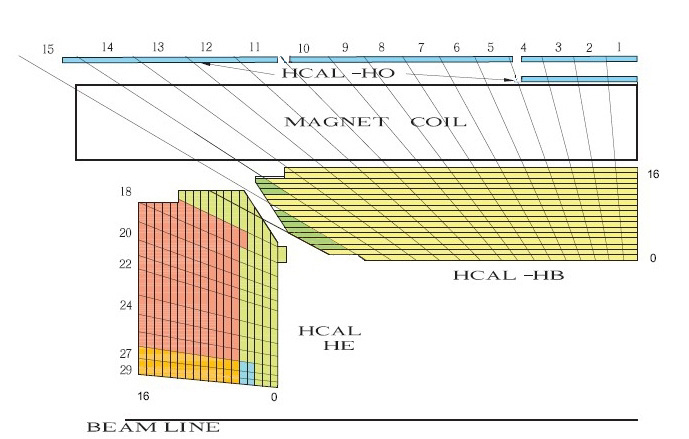
\includegraphics[width=0.75\textwidth]{images/HCAL.jpg}
  	\caption[HCAL Layout]
   	{CMS Hadronic Calorimeter Layout}
	\label{fig:HCALLayout}
\end{figure}

The barrel and endcap HCALs, HB and HE, are located within the 
solenoid magnet. The HB extends across $|\eta|<1.3$ and the HE extends from XXXX
The HB absorber consists of a 40 mm thick front steel plate (which also adds structural integrity),
followed by eight 50.5 mm thick brass plates, six 56.5 mm thick brass plates and
and a 75 mm thick steel plate. At an incident angle of 90$^{\o}$ this corresponds %%fix this
to 5.82 $\lambda_{I}$ while at $\eta$ = 1.3 it corresponds to 10.6 $\lambda_{I}$.
The electromagnetic calorimeter adds another 1.1 $\lambda_{I}$ of additional
material. The HE has a similar design, except the plates have a thickness of 79 mm.
Layered between the absorber plates the plastic scintillator tiles are placed. The 
CMS hadron calorimeter consists of approximately 70,000 tiles which are grouped
into mechanical tray units to ease testing and installation.  
The granularity of the HCAL in $\Delta\eta \times \Delta\phi = 0.087 \times 0.087$
for $|\eta|<1.6$ and $\Delta\eta \times \Delta\phi \approx 0.17 \times 0.17$ for $|\eta|\ge1.6$
The HO is located outside of the solenoid; this means the magnet then acts as an absorbing
medium which contributes an additional 1.4 $\lambda_{I}$. The HO consists of two 
scintillator layers that have the same granularity as the HB. 

The light produced in the scintillators is collected by optical wavelength shifting fibers 
and transferred to Hybrid Photo Diodes (HPDs). HPDs were chosen as the photodetectors
due to their low sensitivity to magnetic fields, %they consist of a photo-cathode held at a HV  Continue this???

The HF is located in the far forward region at $3<|\eta|<5$ and a distance
of  11.2 meters from the interaction point, on average 760 GeV per 
proton-proton interaction is deposited into the forward calorimeters, compared
to an average of 100 GeV in the rest of the detector. This environment
presented a considerable challenge to the calorimetry design. Due to these 
environmental demands the HF is based on radiation hard Cherenkov Quartz technology
which uses quartz fibers as the active medium that are embedded in a steel absorber. 
A signal is generated when charged particles above the Cherenkov threshold %%%fix this
generate light that is then captured by photomultipliers. Therefore, the HF is
more sensitive to electromagnetic showers and relativistic charged pions.
%%%write about resolution



